

\usetikzlibrary{decorations.pathmorphing}
\usetikzlibrary{decorations.text}
\tikzset{
cross/.style={cross out, draw=black, minimum size=2*(#1-\pgflinewidth), inner sep=0pt, outer sep=0pt},
%     %default radius will be 1pt. 
cross/.default={3.5pt}
dot/.style={circle, fill=#1, inner sep=0, minimum size=4pt},
mini dot/.style={circle, inner sep=0pt, minimum size=2pt, pos=1, fill, node contents={}},
}
\begin{center}
 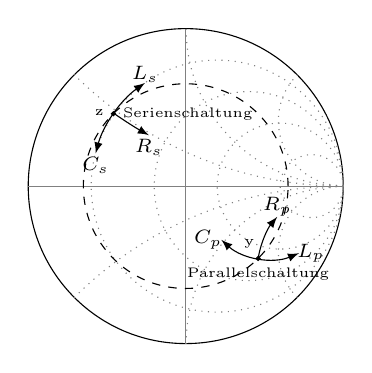
\begin{tikzpicture}    
    
    %Außenkreis
    \draw[-](0,0) circle (2);

    %Realteil Linien
    \draw[-, black!50](-2,0)--(2,0);

    \draw[dotted, black!50](0.4,0) circle (1.6);
    \draw[dotted, black!50](0.8,0) circle (1.2);
    \draw[dotted, black!50](1.2,0) circle (0.8);
    \draw[dotted, black!50](1.6,0) circle (0.4); 

    
    %Imaginärteil Linien
    \draw[-, black!50](0,-2)--(0,2);

    \draw[dotted, black!50, xshift = 13.25ex, yshift = -31.98ex](135:4.84)arc(135:90:4.84);
    \draw[dotted, black!50, xshift = 13.25ex, yshift = -13.25ex](180:2)   arc(180:90:2);
    \draw[dotted, black!50, xshift = 13.25ex, yshift = -5.485ex](225:.828)arc(225:90:.828);

    \draw[dotted, black!50, xshift = 13.25ex, yshift = 31.98ex](270:4.84)arc(270:225:4.84);
    \draw[dotted, black!50, xshift = 13.25ex, yshift = 13.25ex](270:2)   arc(270:180:2);
    \draw[dotted, black!50, xshift = 13.25ex, yshift = 5.485ex](270:.828)arc(270:135:.828);

    %Reflexionsfaktorkreis
    \draw[dashed](0,0) circle (1.3);

    %Serienschaltung
    \draw[-,fill=black!100] (-.919,.919) circle (0.025)node[left, yshift =.5] {\tiny z}node[right]{\tiny Serienschaltung};
    \draw[latex-latex, xshift = 2.65ex](125:1.6)node[above, yshift=-.75ex]{\scriptsize${L_s}$} arc (125:165:1.6)node[below, yshift=.5ex]{\scriptsize$C_s$};
    \draw[latex-, xshift = 13.25ex, yshift = 33.75ex](241:5.1)node[below, yshift=.5ex]{\scriptsize$R_s$}arc(241:235:5.1);

    %Parallelschaltung
    \draw[-,fill=black!100] (.919,-.919) circle (0.025)node[above left, xshift = .5ex]{\tiny y} node[below]{\tiny Parallelschaltung};
    \draw[-latex, xshift = 13.25ex, yshift = -7.25ex](170:1.1)arc(170:140:1.1)node[above, yshift=-.75ex]{\scriptsize$R_p$};

    \draw[latex-latex, xshift = 7.12ex](293:.925)node[right, xshift = -.95ex]{\scriptsize$L_p$}arc(293:227.5:.925)node[left, xshift = .85ex]{\scriptsize$C_p$};

\end{tikzpicture}
\end{center}